\documentclass[../AnalysisNoteJBuxton.tex]{subfiles}
\begin{document}

\subsection{Pair Selection}
\label{PairSelection}

Some general remarks on forming pairs

It is important to obtain true particle pairs in the analysis.  In particular, contamination from pairs constructed with split or merged tracks can introduce an artificial signal into the correlation function, obscuring the actual physics.

\begin{figure}[h]
  \centering
  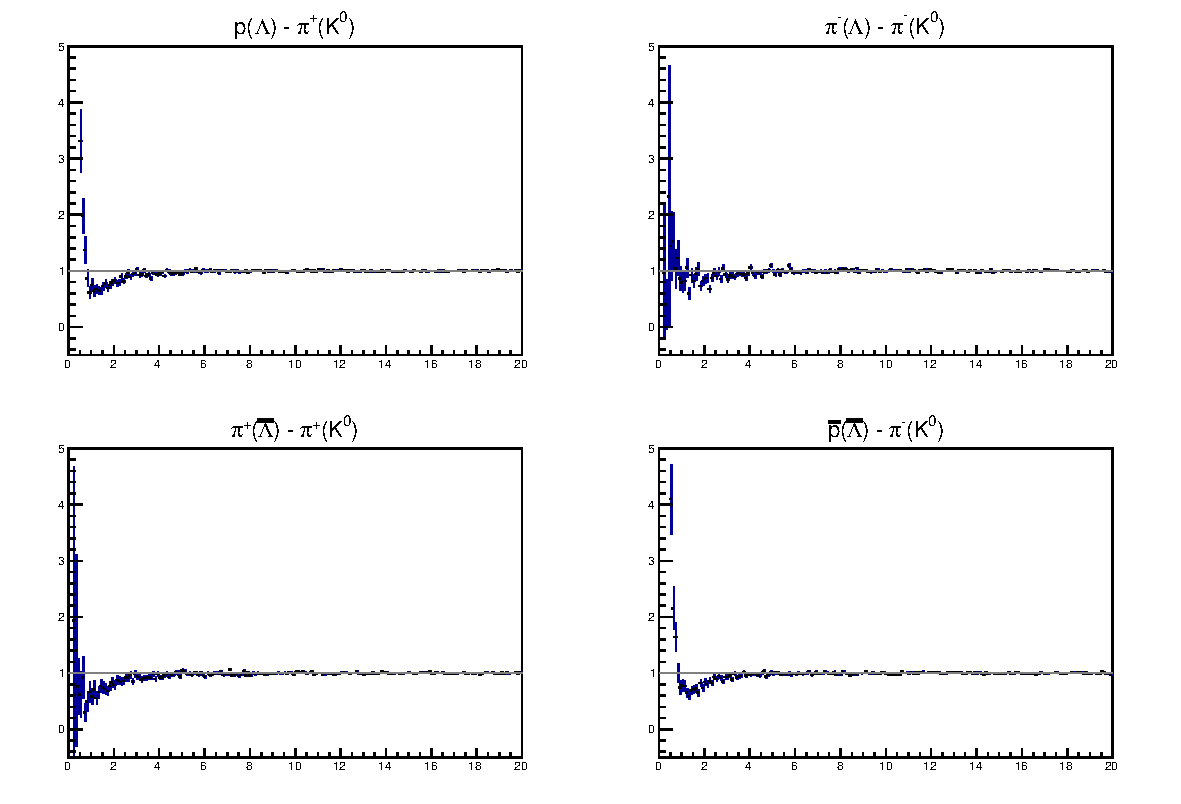
\includegraphics[width=100mm]{3_DataSelection/Figures/AvgSepCFs_LamK0.pdf}
  \caption[Avgerage Separation $\Lambda$($\bar{\Lambda}$)K$^{0}_{S}$]{Avgerage Separation $\Lambda$($\bar{\Lambda}$)K$^{0}_{S}$}
  \label{fig:AvgSepLamK0}
\end{figure}

\begin{figure}[h]
  \centering
  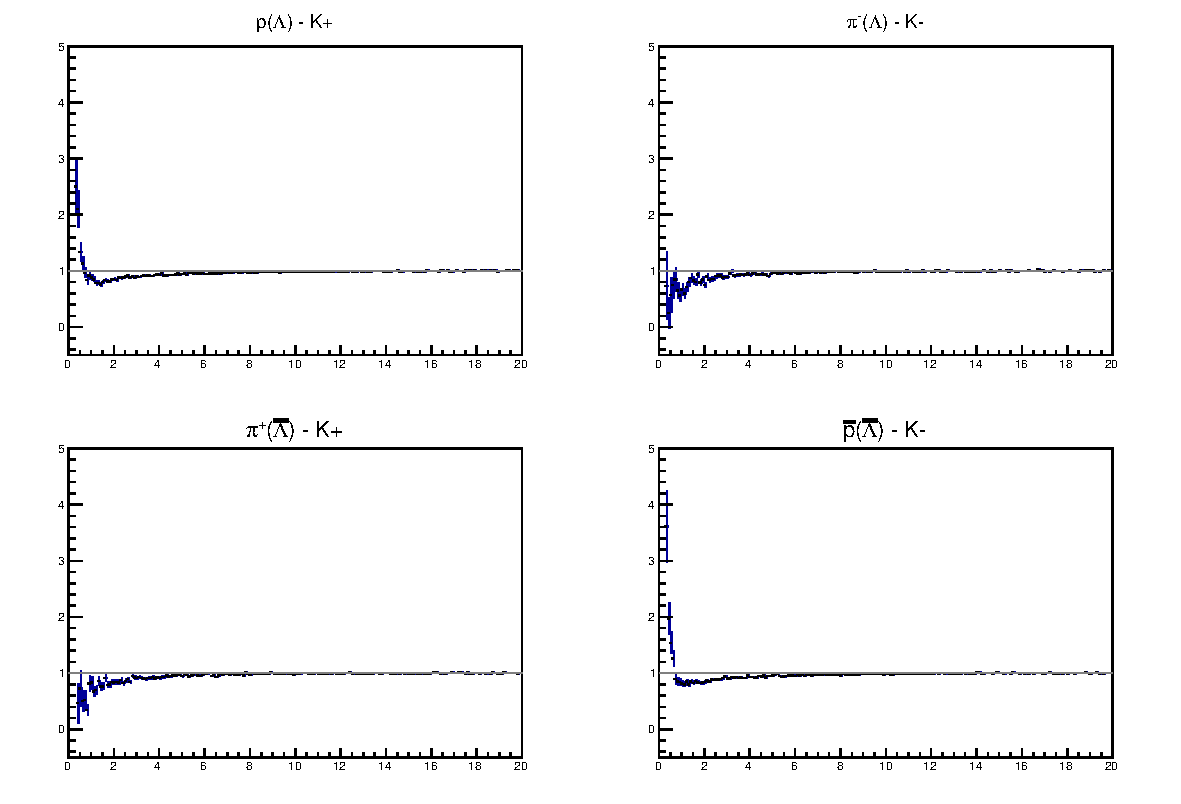
\includegraphics[width=100mm]{3_DataSelection/Figures/AvgSepCFs_LamKch.pdf}
  \caption[Avgerage Separation $\Lambda$($\bar{\Lambda}$)K$^{\pm}$]{Avgerage Separation $\Lambda$($\bar{\Lambda}$)K$^{\pm}$}
  \label{fig:AvgSepLamKch}
\end{figure}

\end{document}